% Working manuscript for the official PVLDB Vol. 20 template.
% Template pin: vldbproceedings/VLDB-Template@39c95f5c6fcbe652a83be24e4eff8f2134cd3fbc
\documentclass[sigconf,nonacm]{acmart}
\usepackage{pvldb}
\usepackage{graphicx}
\usepackage{booktabs}
\usepackage{tabularx}
\usepackage{amsmath}
\usepackage{balance}
\renewcommand\vldbdoi{XX.XX/XXX.XX}
\renewcommand\vldbpages{XXX-XXX}
\renewcommand\vldbavailabilityurl{https://github.com/Doss-com/objectKV}

\newcommand{\okv}{\textsc{objectKV}}
\newcommand{\txlog}{\textit{txLog}}
\newcommand{\codecomplete}{\textsc{[Code Complete]}}
\newcommand{\verified}{\textsc{[Verified]}}
\newcommand{\evaluating}{\textsc{[Evaluating]}}
\newcommand{\proposed}{\textsc{[Proposed]}}
\newcommand{\futurework}{\textsc{[Future]}}
\newcommand{\cversion}{C}
\newcommand{\oversion}{O}

\begin{document}

\title{Constructing objectKV: One Transaction History over Memory, Stable Logs, and Immutable Objects}

\author{Wiley Jones}
\affiliation{%
  \institution{DOSS}
  \city{New York}
  \country{USA}
}
\email{wiley@doss.com}

\begin{abstract}
\okv{} is an open ordered transactional key-value kernel for object-native
data platforms. It separates three concerns that cloud databases often bind
together: transaction ordering, foreground serving, and permanent state. A
bounded cell orders and conflict-checks transactions. A replicated stable-media
transaction log acknowledges durable commits without waiting for object
storage. Disposable RangeEngines serve assigned ranges from RAM, native NVMe,
or RocksDB. Background materializers publish authenticated immutable objects
that support reconstruction, branching, row access, and columnar scans.

This paper describes the target architecture and the measured construction
boundary. The current implementation verifies a topology-matched single-range
RocksDB read path within 12.7\% of direct RocksDB throughput and within 18.4\%
of its p99 through 32 clients. A generation-pinned GCS layout preserved point
p99 while improving a projected scan by 31.692x in a scoped preflight. Complete
GCS recovery reconstructed 25,014 MVCC records with five named GETs and rejected
a one-byte corruption. A TLA+ model explored 264,076 distinct states across two
finite scopes; six weakened-contract controls each reached its named invariant
violation. These results do not establish a complete cell. Independent-machine
quorum latency, multi-range transactions, RAM admission, PostgreSQL, Redis, and
scaled HTAP remain open gates. The contribution is therefore a precise system
shape, evidence boundary, and evaluation program for deciding each layer with
matched controls.
\end{abstract}

\maketitle
\vldbtopmatter

\section{Introduction}

Object storage is an effective capacity and history substrate, but it is a
poor default coordination primitive for latency-sensitive multi-writer
transactions. Point reads also cannot depend on a full restore or an object
request per key. A practical object-native database therefore still needs a
fast foreground path. The architectural question is not whether local state
exists. It is whether local state remains the permanent database, or becomes a
bounded and replaceable accelerator over a reconstructable object base.

\okv{} takes the second position. One cell provides a strict-serializable
ordered KV contract across its ranges. A stable replicated \txlog{} protects
acknowledged mutations. RangeEngines materialize only their assigned working
sets. Immutable object closures hold the portable base, retained history,
branch roots, and scan-oriented projections. PostgreSQL pages, Redis-style
objects, ordered logs, search indexes, virtual filesystems, and DataFusion
tables are intended to meet at one narrow \texttt{okv-fabric} boundary rather
than owning separate consistency domains.

The design is object-native but not object-only. This distinction follows the
same broad physical observation made by cloud database systems such as Aurora,
Socrates, and Neon: log, storage, and compute can be separated without placing
every foreground operation on the capacity tier
\cite{aurora2017,socrates2019,neon2022}. It also adopts FoundationDB's small
ordered transaction API and bounded transaction domain as the semantic target
\cite{fdb2021}, while retaining TiKV and RocksDB as important physical controls
\cite{tidb2020,rocksdb2016}.

The paper makes four contributions:

\begin{itemize}
  \item A bottom-up architecture that separates immutable state, stable commit
  history, disposable serving compute, cell transactions, and typed APIs.
  \item One object layout that aligns row identity, opaque values, columnar
  projection, integrity, and exact recovery without creating two database
  truths.
  \item An executable cell safety model with explicit commit, generation,
  publication, reclamation, and serving invariants.
  \item A governed performance matrix that reports scoped receipts and open
  gates rather than treating code presence as system evidence.
\end{itemize}

\section{Requirements and Status Semantics}

\subsection{Product requirements}

Table~\ref{tab:requirements} fixes the current system intent. The kernel is not
a SQL engine, a Redis clone, or a global metacluster. Those are fabric surfaces
or fleet concerns above a bounded transaction cell.

\begin{table*}[t]
  \centering
  \small
  \caption{System requirements and explicit non-goals.}
  \label{tab:requirements}
  \begin{tabularx}{\textwidth}{@{}p{0.16\textwidth}X X@{}}
    \toprule
    Concern & Requirement & Deliberate boundary \\
    \midrule
    Semantics & Ordered binary keys, point and range reads, snapshots, atomic
    mutation, short strict-serializable transactions & No synchronous
    transaction across cells \\
    Commit & A durable reply requires a declared stable quorum; object
    publication is asynchronous in the default profile & Object storage is not
    the default consensus or acknowledgement service \\
    Serving & Assigned ranges are fast from bounded RAM, native NVMe, or
    RocksDB state & No serving worker owns the only copy of acknowledged data \\
    Persistence & Immutable, generation-pinned S3-compatible closures are
    sufficient for reconstruction with a retained log suffix & No LIST-based
    discovery of authoritative current state \\
    Analytics & One snapshot version feeds row reads and exact columnar
    base-plus-tail queries & Columnar materialization lag may raise query cost,
    but cannot silently lower freshness \\
    Portability & Open object layouts and an engine-neutral fabric permit
    independent compute and storage evolution & No requirement that every hot
    provider share one physical file format \\
    Operations & Cells bound failure radius, recovery generation, version
    space, and capacity & No first-release global distributed transaction or
    autonomous metacluster \\
    \bottomrule
  \end{tabularx}
\end{table*}

\subsection{Evidence vocabulary}

The manuscript uses four statuses. \codecomplete{} means the implementation
exists and its focused checks pass. \verified{} means a named claim has a
retained receipt that binds source, workload, topology, control, evaluator, and
metrics. \evaluating{} means the implementation or evidence is under active
verification. \proposed{} and \futurework{} describe design or later scope.
Every status is local to the stated claim. A verified single-range read does not
verify a cell.

\section{Architecture from Storage Upward}

Figure~\ref{fig:construction} is the compact system map. Permanent bytes sit at
the bottom. Transactions and serving are rebuilt above those bytes. Typed
interfaces sit at the top.

\begin{figure*}[t]
  \centering
  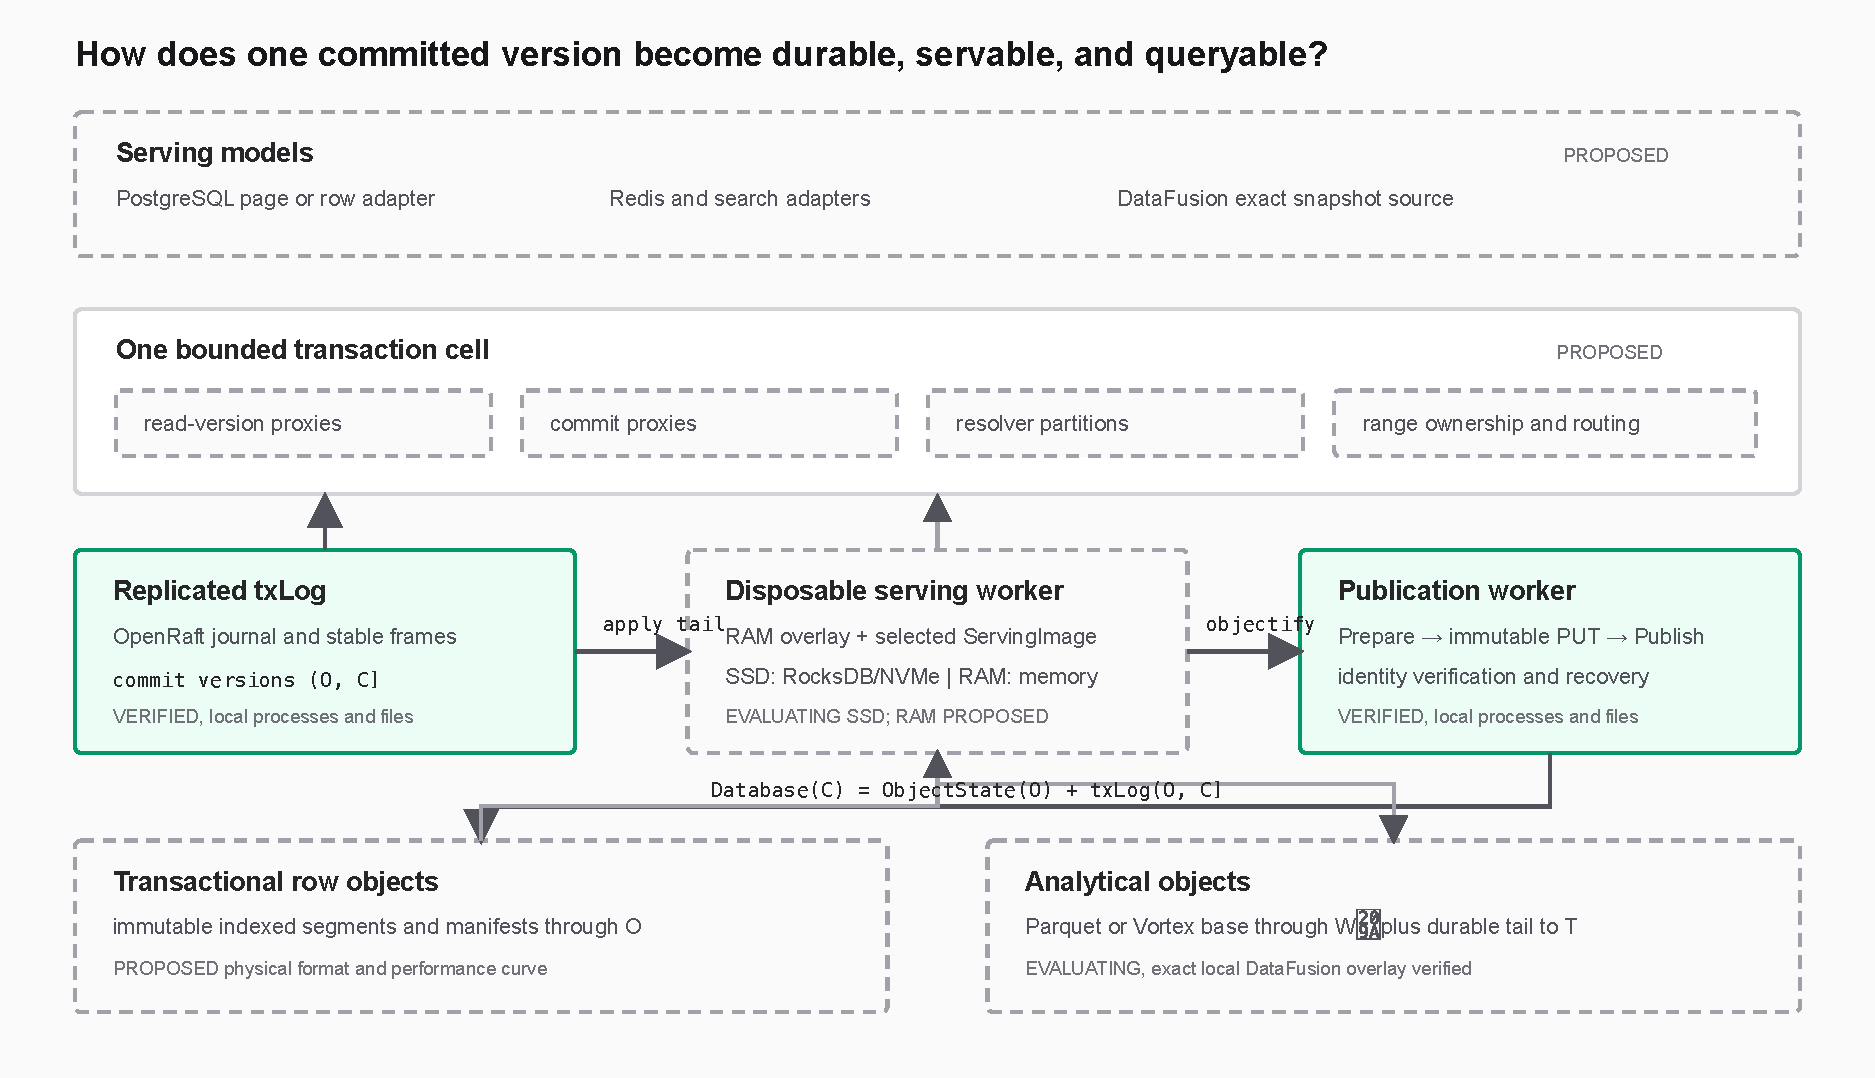
\includegraphics[width=\textwidth]{figures/construction.pdf}
  \caption{\okv{} is one version history with several physical views. Solid
  blue boundaries have scoped implementation evidence. Dashed boundaries are
  target structure.}
  \label{fig:construction}
\end{figure*}

\subsection{Immutable object closure}

The permanent base is a typed root naming a complete immutable closure. The
root binds a generation, child inventory, format versions, logical bounds, and
cryptographic identities. Readers open exact names. Writers create new objects
and atomically activate a new root through the transaction authority. Old roots
remain available while branches, snapshots, backups, queries, or recovery
leases reference them.

Let \cversion{} be the latest committed version and \oversion{} the active
object frontier. The core recovery relationship is:

\begin{equation}
  \oversion \leq \cversion,
  \qquad
  Database(\cversion) = ObjectState(\oversion)
  + StableTxLog(\oversion, \cversion].
  \label{eq:recovery}
\end{equation}

The object closure need not match the in-memory representation. It must preserve
ordered key identity, MVCC history required by policy, integrity, range bounds,
and enough metadata to reconstruct a serving image without searching the
bucket.

\subsection{Stable transaction log}

The \txlog{} is the authoritative suffix of committed mutation outcomes after
\oversion{}. It is not a time log and it is not the application-facing
\texttt{okv-log}. In the default durable profile, a commit is acknowledged only
after a quorum of independent stable media accepts it. Object publication may
continue later. The log prefix can be reclaimed only after the corresponding
object closure is complete, authenticated, active in the same generation, and
protected by every relevant root.

Two higher-level log abstractions build above this boundary:

\begin{description}
  \item[\texttt{okv-log}] An append, read, trim, replay, and branch API for
  applications. Records may contain deterministic semantic operations.
  \item[\texttt{okv-wal}] A recovery-oriented library built on
  \texttt{okv-log}. It adds durable positions, replay rules, checksums, and
  checkpoint references.
\end{description}

Neither abstraction replaces the physical committed-mutation \txlog{} until
crash injection proves equivalent outcomes across software versions.

\subsection{RangeEngine serving compute}

A RangeEngine is the disposable compute runtime for an assigned ordered range.
It owns a recent MVCC overlay, coverage metadata, one chosen resident engine,
read and write budgets, and materialization responsibility. It may use:

\begin{itemize}
  \item \texttt{ram\_image}: an admitted record, block, or complete-range image
  in DRAM;
  \item \texttt{native\_nvme}: a future append-oriented hybrid log and ordered
  index on local NVMe;
  \item \texttt{rocksdb\_image}: a mature disposable ordered image and the
  present verified single-range provider.
\end{itemize}

These are provider choices, not three database truths. A range uses one primary
resident provider at a time, with optional bounded cache above it and an indexed
object miss path below it. Capacity is bounded by assignment and admission.
When the high watermark is reached, the control plane evicts cache, demotes
ranges, splits assignments, or adds workers. Local bytes should scale with the
assigned working set, not total database bytes.

Serving tier and commit depth are independent axes. A RAM image can use quorum
durability; a RocksDB image can run in a relaxed local-only profile; an
object-gated profile can wait for publication. A configuration must name both
its latency shape and its loss envelope.

Garnet reinforces two aspects of this design. Its current implementation opens
typed string, object, unified, and vector sessions over one TsavoriteKV per
logical database, rather than one consistency domain per API
\cite{garnet2025}. Its tiered device also separates hot-to-cold order from the
commit point. \okv{} adopts those structural lessons, but not Garnet's
asynchronous replication or hash-slot transaction boundary.

\subsection{One bounded transaction cell}

A cell is the distributed system, not a page, object, block, or shard.
Figure~\ref{fig:cell} shows the target service topology. One cell has one commit
version space, recovery generation, range map, and stable-log contract. A tenant
transaction may touch arbitrary ranges inside its cell. Cells do not synchronously
coordinate transactions with each other.

\begin{figure*}[t]
  \centering
  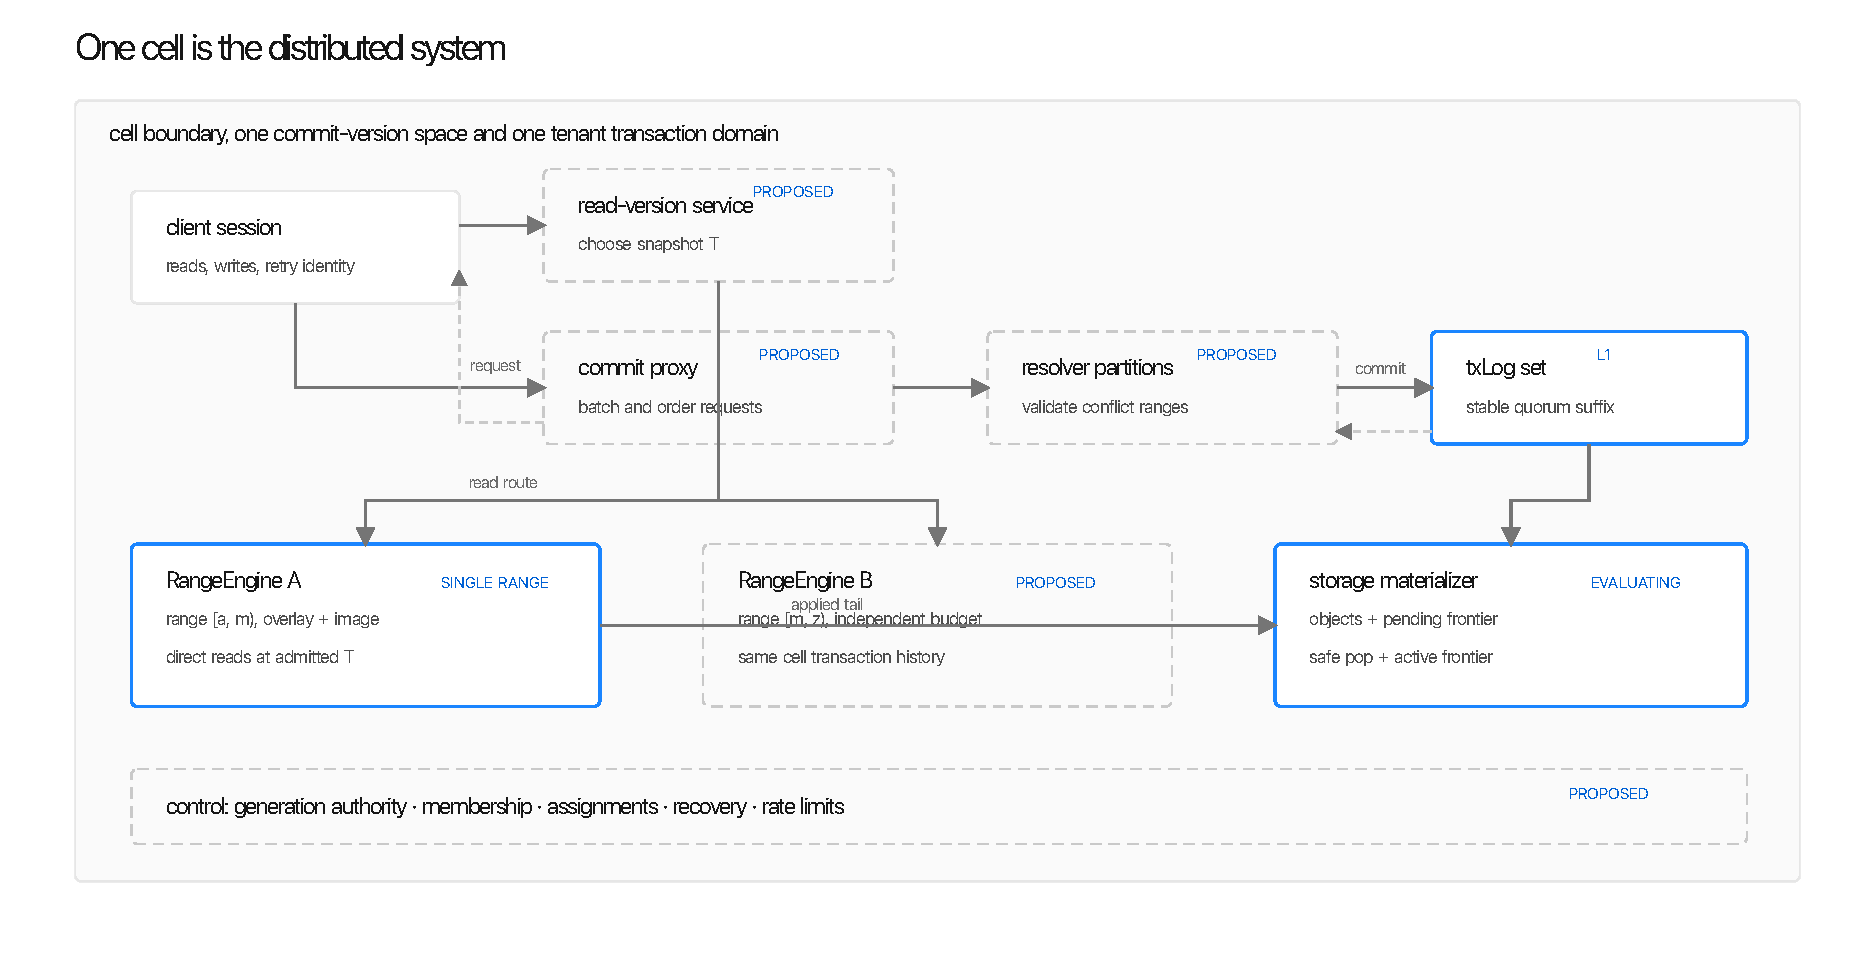
\includegraphics[width=\textwidth]{figures/cell-services.pdf}
  \caption{Target service taxonomy inside one cell. The current implementation
  has single-range serving and one-host log mechanics, not this complete
  distributed topology.}
  \label{fig:cell}
\end{figure*}

The target cell separates five service classes:

\begin{enumerate}
  \item read-version services choose a snapshot version;
  \item commit proxies batch transactions and assign ordered commit work;
  \item resolver partitions validate read and write conflict ranges;
  \item \txlog{} sets make committed outcomes durable;
  \item RangeEngines serve and materialize assigned key ranges.
\end{enumerate}

Generation, membership, assignment, recovery, and rate-limit authorities govern
those services. Initial implementations may co-locate roles, but interfaces
must preserve the separation so measured bottlenecks can later be partitioned.

\subsection{okv-fabric}

The fabric is the shared application boundary over one RangeEngine state. Its
candidate narrow waist is:

\begin{center}
\texttt{read, upsert, atomic\_modify, delete, ordered\_scan}
\end{center}

Operations run inside an explicit transaction or snapshot envelope. Typed views
compile above the waist: bytes and pages for PostgreSQL, structured values for a
Redis-like surface, ordered records for logs and inverted indexes, inode and
extent records for a virtual filesystem, and Arrow batches for analytical
compute. Direct session-to-engine execution is a candidate fast path. Per-core
dispatch remains an alternative that must justify its queue, copy, and context
switch costs.

\section{Foreground and Background Protocols}

Figure~\ref{fig:paths} places commit, point-read, and analytical work side by
side. A useful implementation keeps their foreground dependencies distinct.

\begin{figure*}[t]
  \centering
  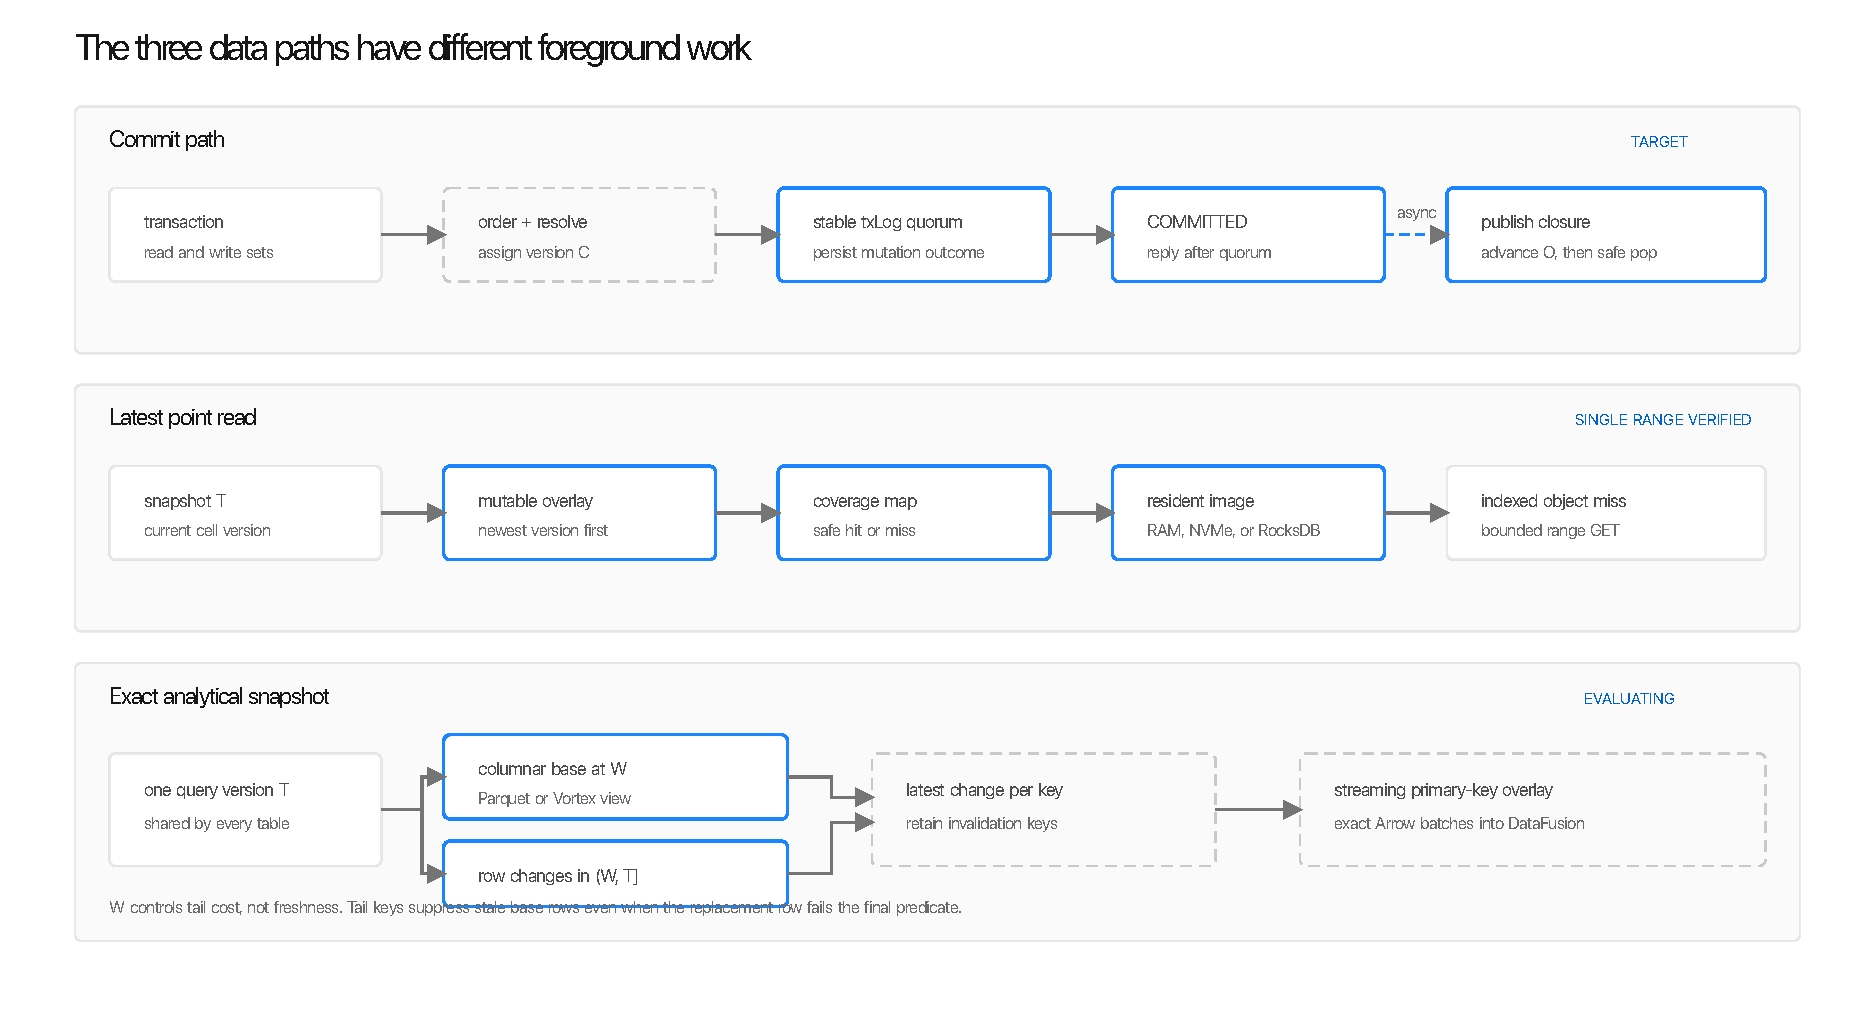
\includegraphics[width=\textwidth]{figures/data-paths.pdf}
  \caption{Foreground dependencies for the three main data paths. The default
  commit does not wait for object publication. A resident point hit issues no
  object request. An analytical query combines a column base with an exact
  invalidating tail.}
  \label{fig:paths}
\end{figure*}

\subsection{Commit}

A transaction reads at version $T$, records read conflict ranges, and submits a
bounded mutation set plus an idempotency identity. The commit proxy assigns
ordered work. Resolvers reject a transaction if a committed write after $T$
intersects its read conflict ranges. Accepted mutations receive a unique
version, persist to the required \txlog{} set, and only then return
\texttt{COMMITTED}. RangeEngines apply tagged mutations asynchronously or from
their local log stream. A lost reply is resolved by transaction identity, not by
blindly applying the transaction again.

The physical \txlog{} may group consecutive records into one bounded node
batch. A node validates the batch before mutation, writes every new frame,
performs one shared stable-media sync, and only then advances memory. Each
record becomes committed only after its containing batch reaches the required
node quorum. This trades explicit batching dwell for fsync amortization; dwell
time remains part of the record's acknowledgement latency.

The current TLA+ model captures this order. The complete multi-range protocol,
partitioned conflict representation, and independent-media performance remain
\evaluating{} or \proposed{}.

\subsection{Latest point read}

A latest read chooses $T$, routes to the range assignment, checks the mutable
overlay, and then consults coverage metadata before the resident provider. A
negative lookup is valid only when the provider proves complete coverage through
$T$. Otherwise the RangeEngine follows the generation-pinned root and compact
index to fetch the required immutable frame. It then fills the admitted cache or
resident image without changing logical state.

The fast path is therefore:

\begin{equation}
  Read(k,T) = NewestVisible(Overlay(k,T), Resident(k,T)).
\end{equation}

An object lookup is an explicit miss path. It is not hidden inside every read.

\subsection{Publication and recovery}

A materializer freezes a range interval through version $P$, emits immutable
children, verifies their hashes and logical digest, prepares a frontier update,
and activates it only in the current generation. Log reclamation follows
activation, not upload completion alone. A replacement worker starts from the
active root, hydrates enough state for its assigned range, and replays the
retained suffix through \cversion{}.

Unknown object outcomes are resolved by exact named reads and content digest.
Bucket listing is not an authority. A stale generation cannot publish, pop a log
prefix, or serve a latest read.

\subsection{Exact HTAP snapshot}

For analytical partition $p$, let $W_p$ be its columnar base watermark and $T$
the query snapshot. Exact state is:

\begin{equation}
  Table_p(T)=ColumnarBase_p(W_p)+RowChanges_p(W_p,T].
  \label{eq:htap}
\end{equation}

The tail is reduced to the latest mutation per primary key. A streaming merge
suppresses base rows touched by the tail, emits surviving tail upserts, and
drops deletes. Tail keys are required for invalidation even if their new rows do
not satisfy the final predicate. Predicate pushdown that removes those keys is
incorrect. DataFusion can consume the resulting ordered Arrow batches through a
custom table provider and execution plan \cite{datafusion2024,arrow2016}.

Every table in one query uses the same $T$, although partitions may have
different $W_p$. The watermark controls query cost, not freshness. Long queries
hold immutable-object and delta-retention leases, not open OLTP transactions.
Values used to enforce a frequent transactional invariant should instead be
maintained as transactional projections. Broad ad hoc analytical decisions
require dependency tokens and short revalidation before writing.

\section{C5v2 Object Layout}

A pure row layout makes projected scans fetch opaque values. A pure column
layout can make point reconstruction and high-update MVCC expensive. C5v2 keeps
one authoritative closure but aligns two physical streams: a projection stream
with ordered keys and selected columns, and a payload stream with opaque values
and tombstones. The compact index maps keys and ranges to aligned frame groups.

\begin{figure*}[t]
  \centering
  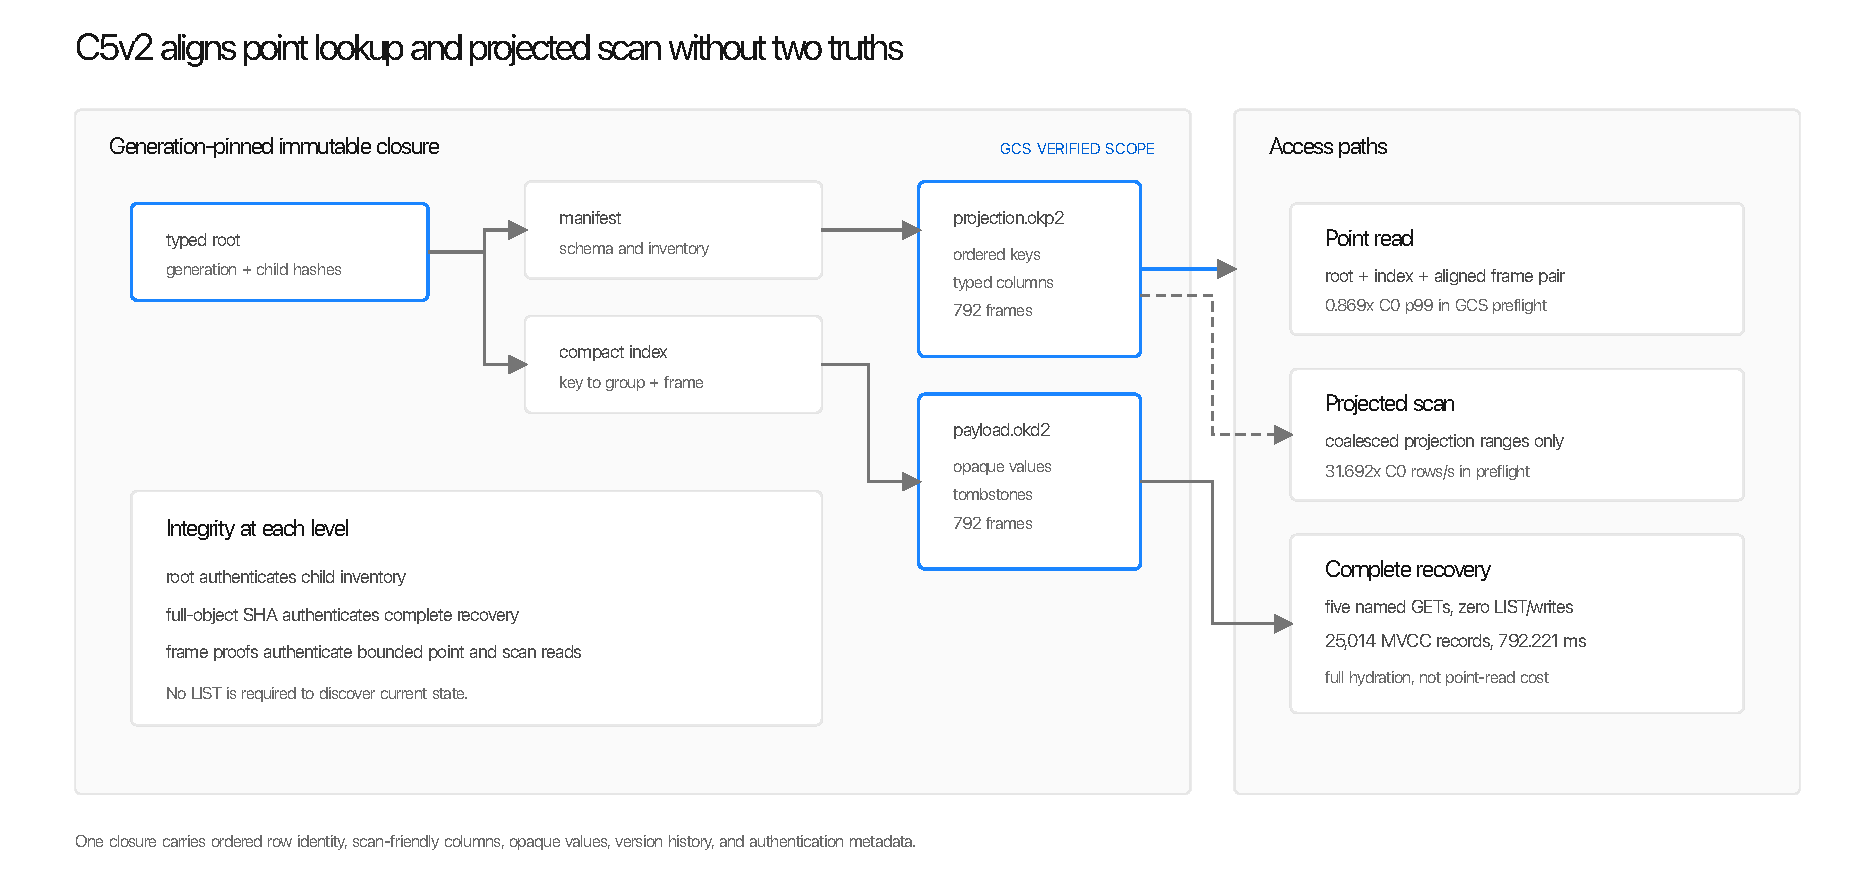
\includegraphics[width=\textwidth]{figures/c5v2-layout.pdf}
  \caption{The C5v2 closure supports bounded point reads, projection-only scans,
  and complete authenticated reconstruction.}
  \label{fig:c5v2}
\end{figure*}

Point lookups use the compact index and fetch the required aligned frame pair.
Projection scans coalesce range requests and avoid payload bytes. Complete
recovery fetches and authenticates every named child. A frame contains enough
version and key identity to reproduce the logical MVCC oracle. This approach
resembles the broader HTAP lesson from HANA that columnar primary storage can
serve transactional work when delta handling and access paths are designed
together \cite{hana2012,hananse2019}. It does not imply that the present layout
is ready to replace a resident point engine.

The layout is format-pluggable above its logical contract. Parquet is a broad
interchange and scan format \cite{parquet}; Vortex and Lance explore lower-latency
random access and richer structural encodings \cite{vortexformat,lance2025}.
Selection must follow a matched point, scan, compaction, and recovery curve, not
format preference.

\section{Executable Safety Contract}

\subsection{Model boundary}

\texttt{ObjectKVCell.tla} is the compact protocol contract for one cell. Its
actions cover transaction begin and sequencing, RAM staging, stable quorum
persistence, commit delivery, generation change, immutable closure construction,
frontier preparation and activation, safe \txlog{} pop, media loss, image
hydration, and reads.

The main invariants are:

\begin{itemize}
  \item \texttt{RepliesTellTheTruth}: committed replies require stable quorum;
  \item \texttt{GenerationsAreFenced}: stale generations cannot commit or serve;
  \item \texttt{PublicationsAreComplete}: active roots name complete closures;
  \item \texttt{SafeTxLogPop}: reclaimed history is protected by the active
  object frontier;
  \item \texttt{ServingReadsAreSafe}: latest reads use a reconstructable,
  current-generation image;
  \item \texttt{ConflictsAreValidated}: conflicting transactions do not both
  commit.
\end{itemize}

The model abstracts consensus to quorum intersection and generation fencing. It
does not prove Raft, Paxos, object storage, RocksDB, liveness, unbounded scale,
or SQL semantics. This composition follows Oswald's useful practice of modeling
log, snapshots, garbage collection, and concurrent actors together, while using
a different acknowledgement boundary \cite{oswald2026}.

\subsection{Finite-state results}

Table~\ref{tab:tla} reports TLC 2.19 using \texttt{tla2tools} 1.7.4 for model
SHA-256 \texttt{55d5bb137b9e...}. TLC found no invariant violation in the two
named finite scopes. Every weakened-contract control reached its exact named
invariant violation and did not terminate on a parser, semantic, or incomplete
successor error.

\begin{table*}[t]
  \centering
  \small
  \caption{Executable model results. Healthy scopes are exhaustive only within
  the listed constants.}
  \label{tab:tla}
  \begin{tabularx}{\textwidth}{@{}p{0.24\textwidth}X r r r l@{}}
    \toprule
    Configuration & Scope or expected violation & Generated & Distinct & Depth & Result \\
    \midrule
    Integrated & 3 nodes, 1 transaction, 2 generations, 1 media failure &
    2,484,568 & 99,408 & 23 & \verified \\
    Concurrency & 3 nodes, 2 conflicting transactions, 2 generations &
    4,496,463 & 164,668 & 28 & \verified \\
    Ack before quorum & \texttt{RepliesTellTheTruth} & 157 & 71 & 5 & poison hit \\
    Ignore generation fence & \texttt{GenerationsAreFenced} & 10,793 & 1,468 & 9 & poison hit \\
    Pop stale frontier & \texttt{SafeTxLogPop} & 82,551 & 7,963 & 12 & poison hit \\
    Publish incomplete closure & \texttt{PublicationsAreComplete} & 13,418 & 1,738 & 9 & poison hit \\
    Serve stale image & \texttt{ServingReadsAreSafe} & 1,483 & 302 & 6 & poison hit \\
    Skip conflict validation & \texttt{ConflictsAreValidated} & 220,294 & 15,475 & 15 & poison hit \\
    \bottomrule
  \end{tabularx}
\end{table*}

A hand-written Rust trace checker replays selected events, verifies the model
identity, and validates constant assumptions. Three current-model GCP traces
each replayed 36 staged-prefix events and three stable-quorum assertions with
zero anomalies; an early-ack trace was rejected after 15 events. This is
\verified{} for the named prefix, not a mechanical refinement. The trace stops
before transaction commit and delivery; two physical process poisons remain
outside its event vocabulary. Liveness, unbounded correctness, and complete-cell
refinement remain \evaluating{}.

\section{Implementation and Infrastructure Boundary}

Figure~\ref{fig:ladder} separates mechanism evidence from operational evidence.
The project has used real files, MinIO, TCP processes, process kill, GCP local
NVMe, regional GCS, restricted service accounts, and independent OTel exports.
It has not yet run the native commit path across three independent machines and
media.

\begin{figure*}[t]
  \centering
  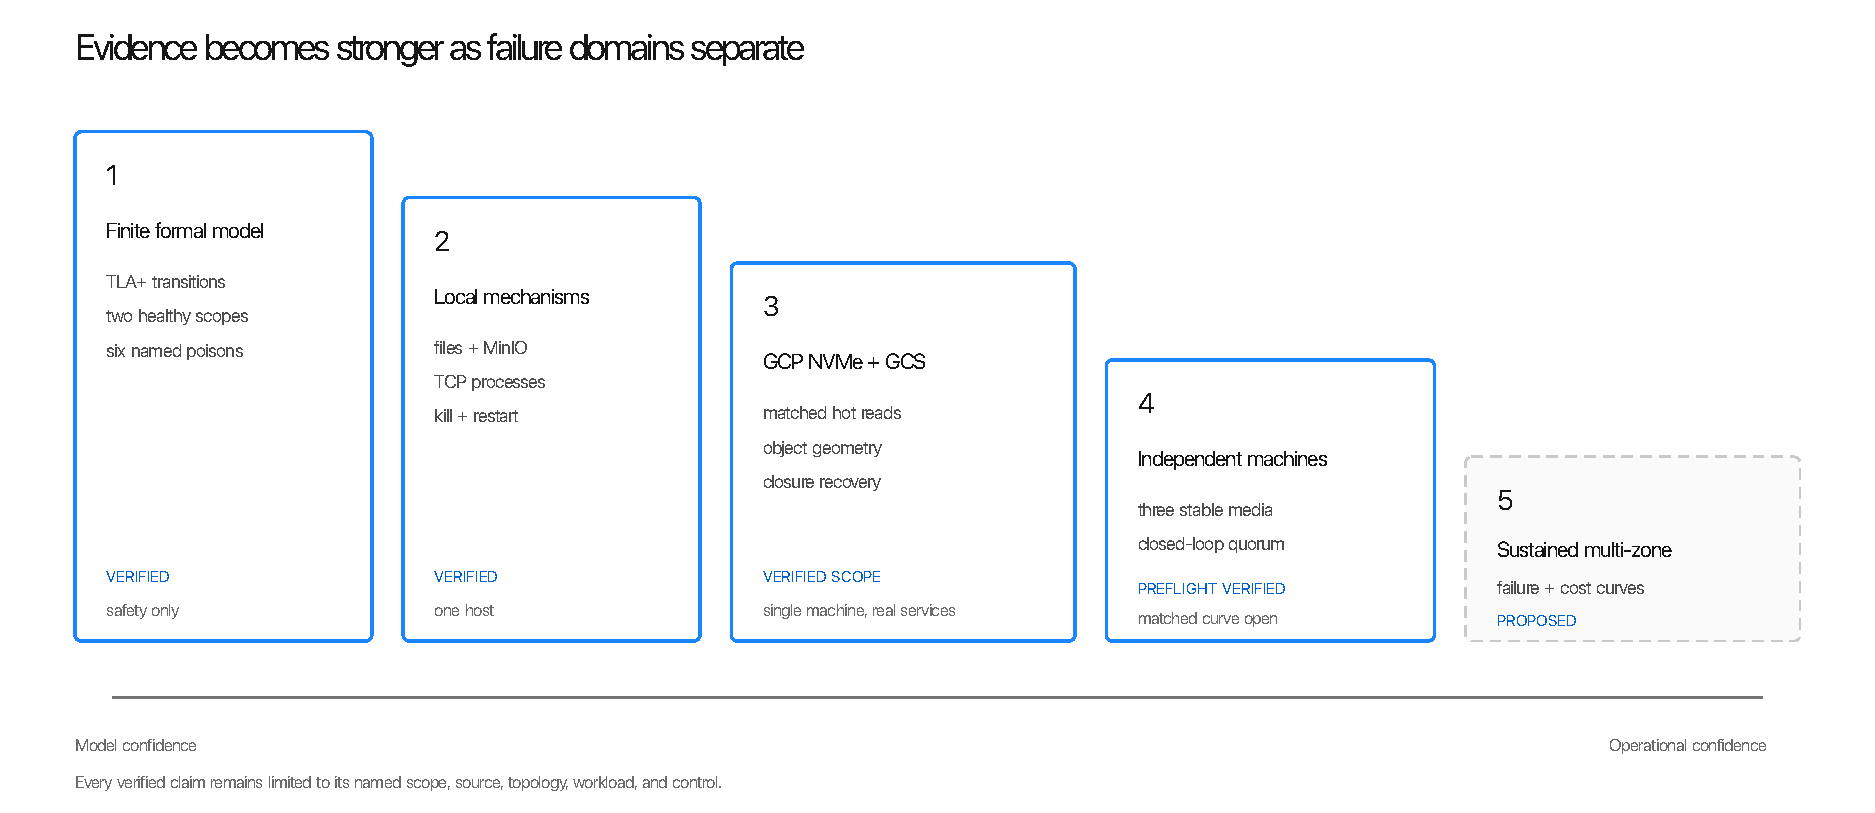
\includegraphics[width=\textwidth]{figures/proof-ladder.pdf}
  \caption{The current evidence ladder. Higher rungs do not inherit lower-rung
  claims unless one receipt composes them.}
  \label{fig:ladder}
\end{figure*}

\begin{table*}[t]
  \centering
  \small
  \caption{Current implementation boundary by subsystem.}
  \label{tab:implementation}
  \begin{tabularx}{\textwidth}{@{}p{0.19\textwidth}p{0.15\textwidth}X X@{}}
    \toprule
    Subsystem & Status & Current evidence & Missing evidence \\
    \midrule
    Ordered MVCC and log primitives & \verified & Deterministic semantics,
    replay, branches, Tetris and Chess state histories & distributed integration
    and compatibility policy \\
    RocksDB RangeEngine & \verified{} scoped & matched single-range reads at 1,
    8, and 32 clients on GCP local NVMe & writes, eviction curve, range movement,
    and full cell RPC \\
    Native quorum \txlog{} & \evaluating & three real TCP processes on one host,
    restart, torn-tail repair, epoch fencing, current-model staged trace & three
    independent machines, matched durable control, integrated transaction \\
    Object publication and recovery & \verified{} scoped & generation-pinned GCS
    root, exact closure reconstruction, corruption rejection, zero-copy branch &
    sustained debt, brownout, publication latency \\
    C5v2 object layout & \evaluating & point and scan GCS preflight, complete
    recovery, 1.040058x compaction bytes & independent OTel, sealed full-curve
    verdict, and write path \\
    Cell transaction plane & \proposed & executable safety model and component
    protocols & complete resolver, proxy, assignment, and multi-range runtime \\
    RAM RangeEngine & \proposed & local playground replay only & matched Garnet,
    SSD, recovery, memory, and cost curves \\
    PostgreSQL, Redis, HTAP & \proposed{} / \evaluating & isolated log primitives
    and bounded DataFusion overlay & end-to-end engines and workload admissions \\
    \bottomrule
  \end{tabularx}
\end{table*}

\section{Evaluation}

\subsection{Method}

Every admitted point names the source and evaluator binary, dataset, payload
distribution, warm or cold state, concurrency, storage devices, object-store
authority, durability depth, process order, control, and OTel identity. AB and
BA ordering limits process-order bias. Negative controls corrupt or weaken one
specific contract and must fail at the named boundary. Ratios are reported only
against matched semantics and topology.

The present results measure isolated mechanisms. They must not be multiplied or
averaged into a complete-stack score.

\subsection{Resident hot read}

The admitted native provider and direct RocksDB control both return owned values
inside the same recovered topology. At one client, native throughput ratios were
0.909x and 0.920x; p99 was 0.913x in both orders. At 8 clients, throughput was
0.880x and 0.873x; p99 was 1.184x and 1.122x. At 32 clients, throughput was
0.880x and 0.891x; p99 was 1.107x and 1.148x. All points passed the declared
0.80 throughput and 1.20 p99 bounds and issued zero measured object operations.

This result says the RangeEngine abstraction can preserve local ordered-read
performance at one bounded scale. It says nothing about replicated commit,
multi-range routing, eviction, or SQL execution.

\subsection{Cache-tail diagnostic}

A later ten-position provider-v2 diagnostic measured native-to-control p50,
p95, p99, and p99.9 ratios of 1.026x, 1.131x, 1.742x, and 1.032x. The p99 result
misses the 1.20 gate. Because adjacent percentiles and the resident-footprint
checks passed, the program records this as an explicit tail-attribution debt and
moves to higher-value system gates. It is not an admitted cache curve.

\subsection{Object layout and recovery}

The C5v2 GCS viewer-only preflight measured 0.869x the C0 point-read p99,
31.692x the C0 projection-scan throughput, and 1.043x its object bytes. A larger
curve completed all positions but its evaluator-only replay names did not match,
so no sealed curve verdict is claimed.

Complete-child recovery fetched the typed root and four children using five full
GETs, 13,700,110 response bytes, zero range GETs, zero LIST, and zero writes. It
verified 792 projection and 792 payload proofs, reconstructed 25,014 MVCC records
and 15,742 live rows, and completed in 792.221 ms. A cloud poison changed byte
zero of the exact projection object and recovery rejected it at the
generation-pinned child SHA boundary after the same five-GET graph.

A separate real-GCS media run created one 4,344-byte branch root that reused
26,820,839 bytes of exact parent children with zero child-object PUTs. Six C5v2
runs wrote 27,304,907 provider-accounted bytes through 24 create-only PUTs,
1.040058x the deterministic C0 control and below the frozen 1.10x ceiling. It
used zero LIST requests and reopened the compacted four-object closure to
reproduce the exact 25,014-record history. This verifies media geometry, not
publication latency or independent telemetry.

\begin{figure*}[t]
  \centering
  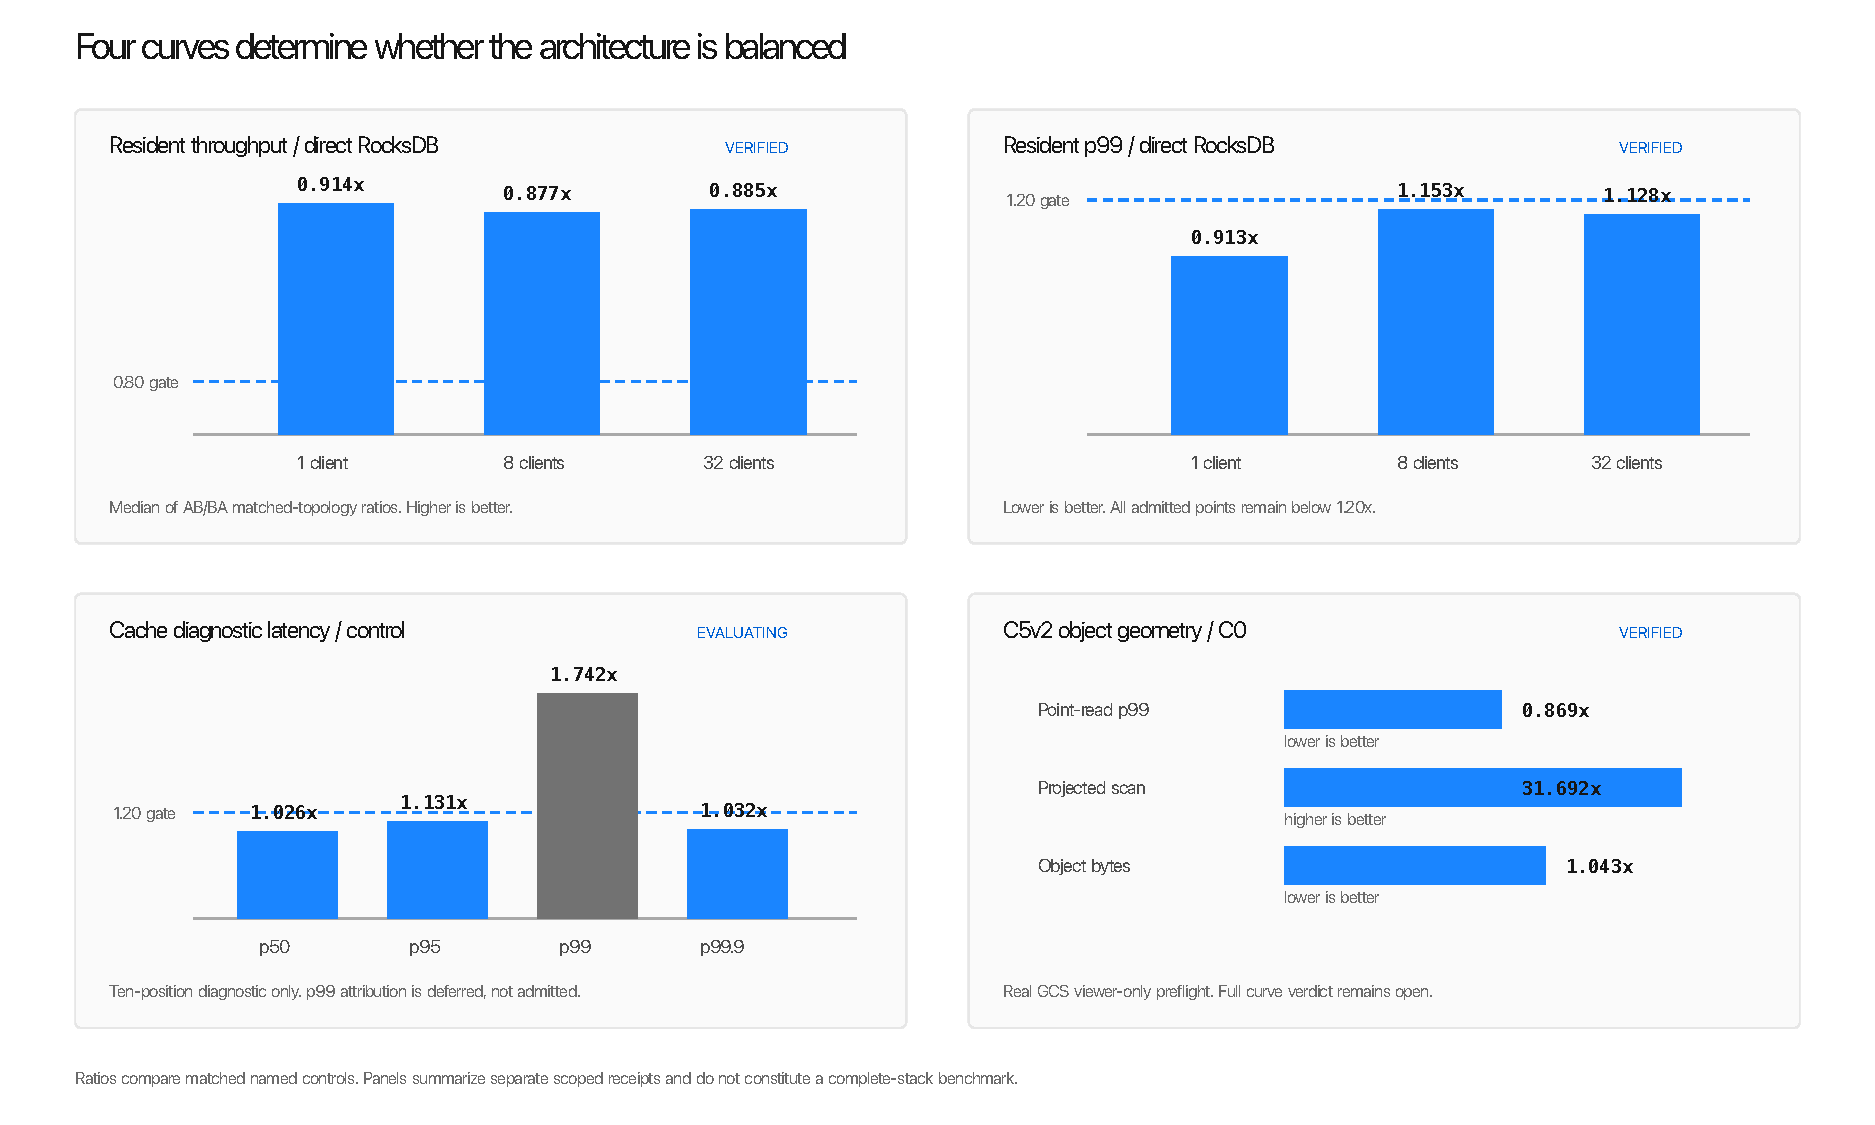
\includegraphics[width=\textwidth]{figures/performance-balance.pdf}
  \caption{Four currently decision-bearing curves. Each panel has its own
  workload and status.}
  \label{fig:performance}
\end{figure*}

\subsection{Performance matrix}

Table~\ref{tab:matrix} is the program's rowing machine. Each row admits one
additional system claim. Work moves upward only when the current row exposes no
more important blocker than the next row.

\begin{table*}[t]
  \centering
  \scriptsize
  \caption{Master performance matrix, 2026-08-30.}
  \label{tab:matrix}
  \begin{tabularx}{\textwidth}{@{}r p{0.22\textwidth}p{0.13\textwidth}X X@{}}
    \toprule
    Row & Curve & Status & Strongest current evidence & Next decision-bearing gate \\
    \midrule
    0 & Resident NVMe point read & \verified & 0.873x to 0.920x RocksDB
    throughput; p99 0.913x to 1.184x & retain as regression control \\
    1 & Cache coverage and eviction & \evaluating & footprint corrected; diagnostic
    p99 1.742x & attribute hit and miss samples before resuming frozen sweep \\
    2 & Cold indexed point read & \evaluating & one bounded range GET; provider tail
    missed two block gates & return after object-layout write path \\
    3 & Point and scan object geometry & \evaluating & C5v2 preflight, recovery,
    1.040058x compaction bytes, and zero-copy branch verified & independent OTel
    and sealed curve verdict \\
    4 & Native three-node commit & \evaluating & one-host TCP log mechanics,
    finite TLA+ safety, current-model staged trace & three independent NVMe
    machines versus matched control \\
    5 & Brownout and host loss & \evaluating & exact base plus suffix recovery &
    sustained write with object-fault schedule and hard debt ceiling \\
    6 & Branch and lazy reopen & \evaluating & exact local branch and empty worker &
    parent-size sweep with GCS request accounting \\
    7 & Multi-range cell & \proposed & no admitted runtime & strict-serializable
    cross-range history, then 1, 2, 4, 8 range groups \\
    8 & RAM serving and handoff & \proposed & playground semantics only & require a
    20\% gain on one declared end-to-end metric \\
    9 & Log, Redis, search, and VFS fabric & \proposed & local \texttt{okv-log}
    game histories & one semantic oracle and one specialist curve per surface \\
    10 & PostgreSQL page OLTP & \proposed & page boundary documented & first adapter
    within 2x local PostgreSQL, then resident target within 1.25x \\
    11 & DataFusion exact HTAP & \evaluating & exact bounded overlay; isolated source
    2.544M rows/s & tails at 0, 0.1, 1, and 10\% plus OLTP interference \\
    12 & Complete-stack economics & \proposed & component metrics only & matched
    failure, capacity, request, compute, and operator cost \\
    \bottomrule
  \end{tabularx}
\end{table*}

\section{Architectural Decisions and Tradeoffs}

\subsection{Why not an object-only WAL?}

Object-gated commits simplify the durability story but place object latency,
availability, request throttling, and often single-region assumptions directly
on every acknowledgement. Batching restores throughput at the cost of latency
and leader machinery. The default \okv{} profile instead uses a stable quorum
for the foreground suffix and asynchronous immutable publication. This adds a
log service and objectification debt, but makes that debt visible and bounded.
An object-committed profile remains possible when its latency and regional loss
contract is acceptable.

\subsection{Why not FoundationDB plus objects?}

FoundationDB already supplies a mature transaction plane and remains the
strict-serializability oracle and fallback. Pairing it with immutable object
history is the fastest route to higher-level product learning. It also retains
a second permanent storage system, keeps placement and recovery coupled to the
FoundationDB fleet, and cannot directly make the open object closure the
reconstruction boundary. The program therefore keeps two lanes: use
FoundationDB to validate semantics and applications, while the native lane must
earn replacement through matched durability and performance gates.

\subsection{Why not rebuild TiKV?}

Recreating TiKV's full Raft, RocksDB, placement, backup, and SQL integration
stack would spend most effort reproducing a mature permanent-replica system.
\okv{} reuses RocksDB today and studies a narrower native log later. Its novel
claim is not a faster RocksDB wrapper. It is bounded disposable range state over
generation-pinned immutable history, with exact row and column views. If local
bytes still scale with database bytes or recovery requires full replica copy,
the distinction disappears and TiKV is the stronger substrate.

\subsection{Raft or Paxos?}

The product contract depends on quorum intersection, fencing, ordered decisions,
and recovery generations, not algorithm branding. Raft provides an understandable
initial implementation and strong library support \cite{raft2014}. A Paxos-family
protocol may later improve reconfiguration or availability topology. The first
three-machine eval should compare a correct, matched durable path before
optimizing consensus variants.

\subsection{RocksDB or a native hybrid log?}

RocksDB is the admitted SSD provider and a durable engineering shortcut. It
brings ordered reads, compaction, bloom filters, cache management, snapshots,
and recovery, but can duplicate \okv{}'s own MVCC, log, and objectification work.
A Garnet-like native hybrid log could unify RAM and NVMe serving, reduce copies,
and make checkpoint phases explicit. It also requires substantial concurrency,
index, eviction, and recovery engineering. The native provider should begin only
with a direct-execution versus dispatch benchmark and a crash matrix for semantic
versus physical logging.

\subsection{Row, page, or column?}

The kernel remains value-native. PostgreSQL can initially treat values as pages,
preserving its buffer manager and page semantics rather than rewriting the
database as a row engine. Redis-like structures and logs can store operation or
object records. C5v2 can derive a scan-efficient projection from the same commit
history. No single physical granularity must dominate every surface. The strict
requirements are one transaction history, exact version alignment, and explicit
amplification.

\section{Risks and Next Evaluations}

\begin{table*}[t]
  \centering
  \small
  \caption{Primary architectural risks and the earliest useful measurement.}
  \label{tab:risks}
  \begin{tabularx}{\textwidth}{@{}p{0.19\textwidth}X X X@{}}
    \toprule
    Risk & Failure signal & Earliest decisive eval & Consequence \\
    \midrule
    Quorum tax & native commit p99 exceeds 1.25x matched durable control after
    one optimization cycle & three independent NVMe machines, exact same
    durability and client path & retain FoundationDB or TiKV transaction plane \\
    Double logging & engine WAL, \txlog{}, and objectification dominate bytes or
    CPU & per-layer bytes and CPU during mixed writes & native hybrid log or
    remove redundant durability layer \\
    Object debt & $\cversion-\oversion$, log bytes, or recovery time grows without
    bound & sustained writer with 30-minute object brownout & hard backpressure,
    more materializers, or reject workload class \\
    Cold-read cliff & requests or metadata bytes grow with total database size &
    10 GiB and 10 M key point and reopen sweep & redesign index and closure \\
    RAM has no role & no 20\% gain over admitted SSD on latency, throughput, or
    CPU after cost normalization & matched Garnet, RAM, and RocksDB subset & keep
    RAM as cache only \\
    HTAP tail cliff & 1\% tail adds more than 20\% or requires unbounded memory &
    exact DataFusion tail sweep with update invalidations & increase
    materialization rate or narrow zero-ETL claim \\
    Operational overreach & repair needs full-cell copy or coupled global
    coordination & host-loss, branch, and range-move fault schedule & shrink cell
    envelope and simplify authorities \\
    \bottomrule
  \end{tabularx}
\end{table*}

The immediate sequence is narrow:

\begin{enumerate}
  \item confirm C5v2 recovery and media accounting in independent OTel;
  \item run the native \txlog{} on three independent NVMe machines against one
  matched remote durable control;
  \item integrate one transaction path only if that curve clears;
  \item then begin the first multi-range strict-serializability history.
\end{enumerate}

This order avoids building PostgreSQL, Redis, and DataFusion product surfaces on
an unmeasured commit and range foundation. It also avoids waiting for every tail
optimization before testing the next architectural mortality risk.

\section{Related Work}

FoundationDB is the primary semantic reference for ordered transactions,
versioned reads, proxies, resolvers, logs, and bounded transaction domains
\cite{fdb2021}. TiDB and TiKV demonstrate the mature alternative of Raft-backed
RocksDB ranges with SQL and analytical replicas \cite{tidb2020}. Aurora,
Socrates, and Neon separate database compute, durable logging, and remote storage
at page and log boundaries \cite{aurora2017,socrates2019,neon2022}.

Garnet and Tsavorite show how a narrow operation waist, direct request
execution, typed views, hybrid logs, and explicit commit depth can produce a
high-performance memory and SSD engine \cite{garnet2025}. CloudJump III studies
RAM, SSD, durable, and object tiers for cloud database execution
\cite{cloudjumpiii2026}. HANA demonstrates transaction processing over columnar
state and piecewise access \cite{hana2012,hananse2019}. Paimon and RisingWave
explore object-backed primary-key and state-store layouts
\cite{paimonpk,paimonpfile,risingwavestore}. \okv{} differs in the proposed
combination of one bounded strict-serializable cell, disposable range serving,
an authenticated immutable reconstruction base, and exact row-column version
alignment.

\section{Conclusion}

The emerging \okv{} vision is a small transactional kernel for data platforms,
not a database product with every feature embedded in the kernel. One cell owns
transactionality. One stable \txlog{} owns the acknowledged suffix. One
RangeEngine state exposes several typed fabric views. Immutable object closures
own portable reconstruction, history, branching, and analytical layout.

Current evidence supports the single-range RocksDB read boundary, scoped C5v2
GCS geometry and recovery, the finite cell safety model, and current-model
staged-prefix trace conformance. It does not yet support the complete
distributed claim. The next useful proof is physical: a
three-machine stable-quorum curve with exact durability and failure controls.
If that path clears, multi-range transactions become the next kernel milestone.
PostgreSQL, Redis-like objects, logs, search, virtual filesystems, and DataFusion
then become typed consumers of one measured fabric rather than separate storage
systems.

\balance
\bibliographystyle{ACM-Reference-Format}
\bibliography{references}

\end{document}
